\chapter{Metodología de la Investigación}

\section{Diseño de la investigación}

Según \cite{bk_sampieri2014metodologia}, los diseños experimentales se caracterizan por manipular y establecer relaciones de causa-efecto entre variables independientes y dependientes.

En esta investigación, se adopta un diseño experimental, ya que se busca establecer una relación entre las técnicas y modelos de aprendizaje profundo, específicamente redes neuronales convolucionales (CNN), y la detección automatizada de deterioros en pavimentos en Lima Metropolitana. Esto implica manipular los parámetros del modelo, así como las características de los datos utilizados, para analizar el impacto en la precisión y efectividad del sistema desarrollado.

\subsection{Tipo de la investigación}

Definido el diseño experimental, el tipo de investigación es experimental puro, ya que la variable independiente (técnicas y modelos de CNN) será manipulada para observar su impacto en la variable dependiente (precisión en la detección de deterioros). Esta manipulación incluye ajustes en los hiperparámetros del modelo, selección de características de las imágenes y técnicas de procesamiento de datos para optimizar los resultados.

Además, se realizarán iteraciones con diferentes configuraciones y subconjuntos del dataset, buscando maximizar métricas como precisión, recall y F1-score, indicadores clave del desempeño del modelo en la tarea de clasificación.

\subsection{Enfoque de la investigación}

De acuerdo con \cite{bk_sampieri2014metodologia}, el enfoque cuantitativo utiliza herramientas estadísticas y sigue un proceso estructurado y secuencial para medir variables y analizar relaciones entre ellas.

Esta investigación sigue un enfoque cuantitativo, ya que los resultados del modelo CNN serán evaluados mediante métricas estadísticas que permiten medir su rendimiento en la clasificación de imágenes de pavimentos. Las métricas empleadas, como precisión, recall, F1-score y curva ROC, servirán para evaluar de manera objetiva la efectividad del sistema propuesto.

\subsection{Población}

La población corresponde a imágenes de pavimentos urbanos en diversas condiciones de conservación, recolectadas en el contexto de la ciudad de Lima Metropolitana. Estas imágenes reflejan una variedad de tipos de deterioro comunes en pavimentos, como grietas y fisuras, que afectan la infraestructura vial.

\subsection{Muestra}

La muestra está constituida por un conjunto de 30,000 imágenes, clasificadas en dos categorías principales: con grietas y sin grietas. Estas imágenes fueron obtenidas por el autor Omoebamije Oluwaseun, utilizando un dron DJI Mavic 2 Enterprise para tomas aéreas y un smartphone para capturas a nivel del suelo. Las imágenes están en formato RGB, resolución 227x227 píxeles, y han sido etiquetadas previamente para su uso en tareas de clasificación mediante CNN.

\section{Alcance de la Investigación}

El alcance de la investigación incluye el diseño, entrenamiento y evaluación de un modelo CNN que permita clasificar imágenes de pavimentos de manera automática. Esto abarca:

Recolección y preparación del conjunto de datos de imágenes.
Implementación de técnicas de preprocesamiento y limpieza de datos.
Entrenamiento de modelos CNN con diferentes configuraciones.
Evaluación de la efectividad del modelo y comparación con métodos tradicionales de inspección visual.
El objetivo principal es contribuir a la optimización del mantenimiento vial, reduciendo costos y mejorando la seguridad vial mediante un sistema automatizado para la detección de deterioros.
\section{Metodología de Implementación de la Solución}
La metodología por seguir para implementar un modelo de Deep Learning está basado en gran medida en el conocido ciclo de vida de desarrollo de modelos de Inteligencia Artificial, del cual gran parte de los antecedentes mostrados anteriormente siguen con algunas variaciones. 

En el presente caso, se pretende desarrollar un modelo de Deep Learning capaz de brindar ayuda en el diagnóstico médico; por tal motivo, se optó por basar metodología de esta investigación en la de \cite{pr_monroy2021disvc}, modificándolo en cierta medida en el contexto de nódulos tiroideos e imágenes de ultrasonido. En la Figura \ref{3:fig301} se presenta de forma gráfica la metodología a seguir.

\begin{figure}[H]
	\begin{center}
		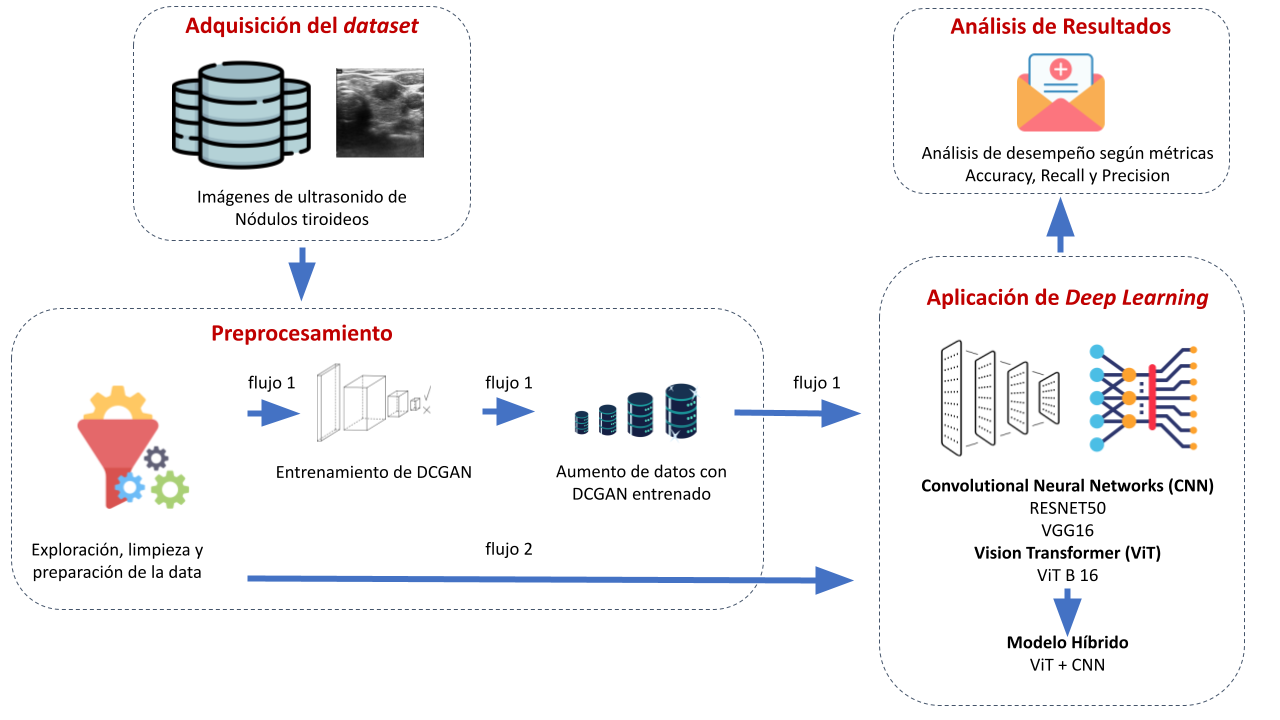
\includegraphics[width=1.00\textwidth]{3/figures/metod_classthy1.png}
		\caption[Metodología de implementación]{Metodología de implementación. \\
		Fuente: Elaboración propia.}
		\label{3:fig301}
	\end{center}
\end{figure}

La adquisición del conjunto de datos, es decir, imágenes de ultrasonido, consiste en la búsqueda y revisión de las bases de datos sobre imágenes de nódulos tiroideos, donde finalmente se seleccionará y descargará la de mayor utilidad. La base de datos debe cumplir con ciertos requerimientos para realizar un posterior entrenamiento del modelo que otorgue buenos resultados. Las imágenes deben ser debidamente etiquetadas según el carácter del nódulo al que representen, es decir, se debe indicar si cada una de las imágenes pertenece a la categoría benigno o maligno. Además, para evitar discrepancias entre calidad de imágenes en futuras evaluaciones, el conjunto de datos debe poseer imágenes de distintas instituciones de salud y de distintas calidades. Esto permitirá que el modelo entrenado no dependa de la una alta o baja calidad de las imágenes para realizar una correcta predicción. Finalmente, la cantidad de datos debe ser relativamente alta con el fin de aumentar la capacidad de generalización del modelo y evitar posibles sobreajustes o bajo rendimiento.  

En la etapa de preprocesamiento, se realizará en primera instancia una exploración del conjunto de datos con el fin de entender su composición y las características a mejorar; por ejemplo, un posible desbalanceo de clases o presencia de imágenes corruptas o sin etiquetar. Posteriormente, se realizará limpieza datos en caso de imágenes corruptas o de nula utilidad. Además, se usarán técnicas de Aumento de Datos en la situación de desbalanceo de datos, con el fin de evitar una baja generalización y sobreajuste en la clase mayoritaria. Además, se aplicará un redimensionamiento y normalización en las imágenes destinadas al entrenamiento del modelo con el objetivo de reducir la complejidad computacional y así obtener menor tiempo de ejecución.

Una vez se tenga la data ya preprocesada, una parte de este se usará para el entrenamiento de modelos de Deep Learning. Inicialmente, se planea usar algunos de los diversos tipos y arquitecturas de Redes Neuronales Convolucionales (CNN), específicamente los más utilizados en este tipo de tareas como lo son VGG y ResNet, pues son ideales para la extracción de características de las imágenes, facilitando así el proceso final de clasificación. Además, se desarrollarán modelos basados en arquitecturas de Vision Transformer debido al potencial que han demostrado en anteriores investigaciones. Finalmente, también se realizará el desarrollo de modelos híbridos de CNN con Vision Transformer. %similares a los descritos por \cite{pr_JERBI2023autoclassViTGAN}.

Cada uno de los modelos será probado en la parte restante de la data, específicamente en la data de prueba o test. De aquí se obtendrán las predicciones de los modelos clasificando las imágenes en benigno (0) o maligno (1).

\section{Metodología para la Medición de Resultados de la Implementación}

Los resultados obtenidos de la clasificación de los modelos previamente entrenados deberán ser evaluados para una correcta elección final. 

Antes de presentar las métricas a usar, es necesario conocer a la matriz de confusión y las partes que lo conforman, pues servirá como base para entenderlas. 

Según \cite{ws_izco2018bdcp} la matriz de confusión es una herramienta que permite ver de forma más clara el rendimiento de nuestro modelo. Este se presenta en la Figura \ref{3:fig302}.

\begin{figure}[H]
	\begin{center}
		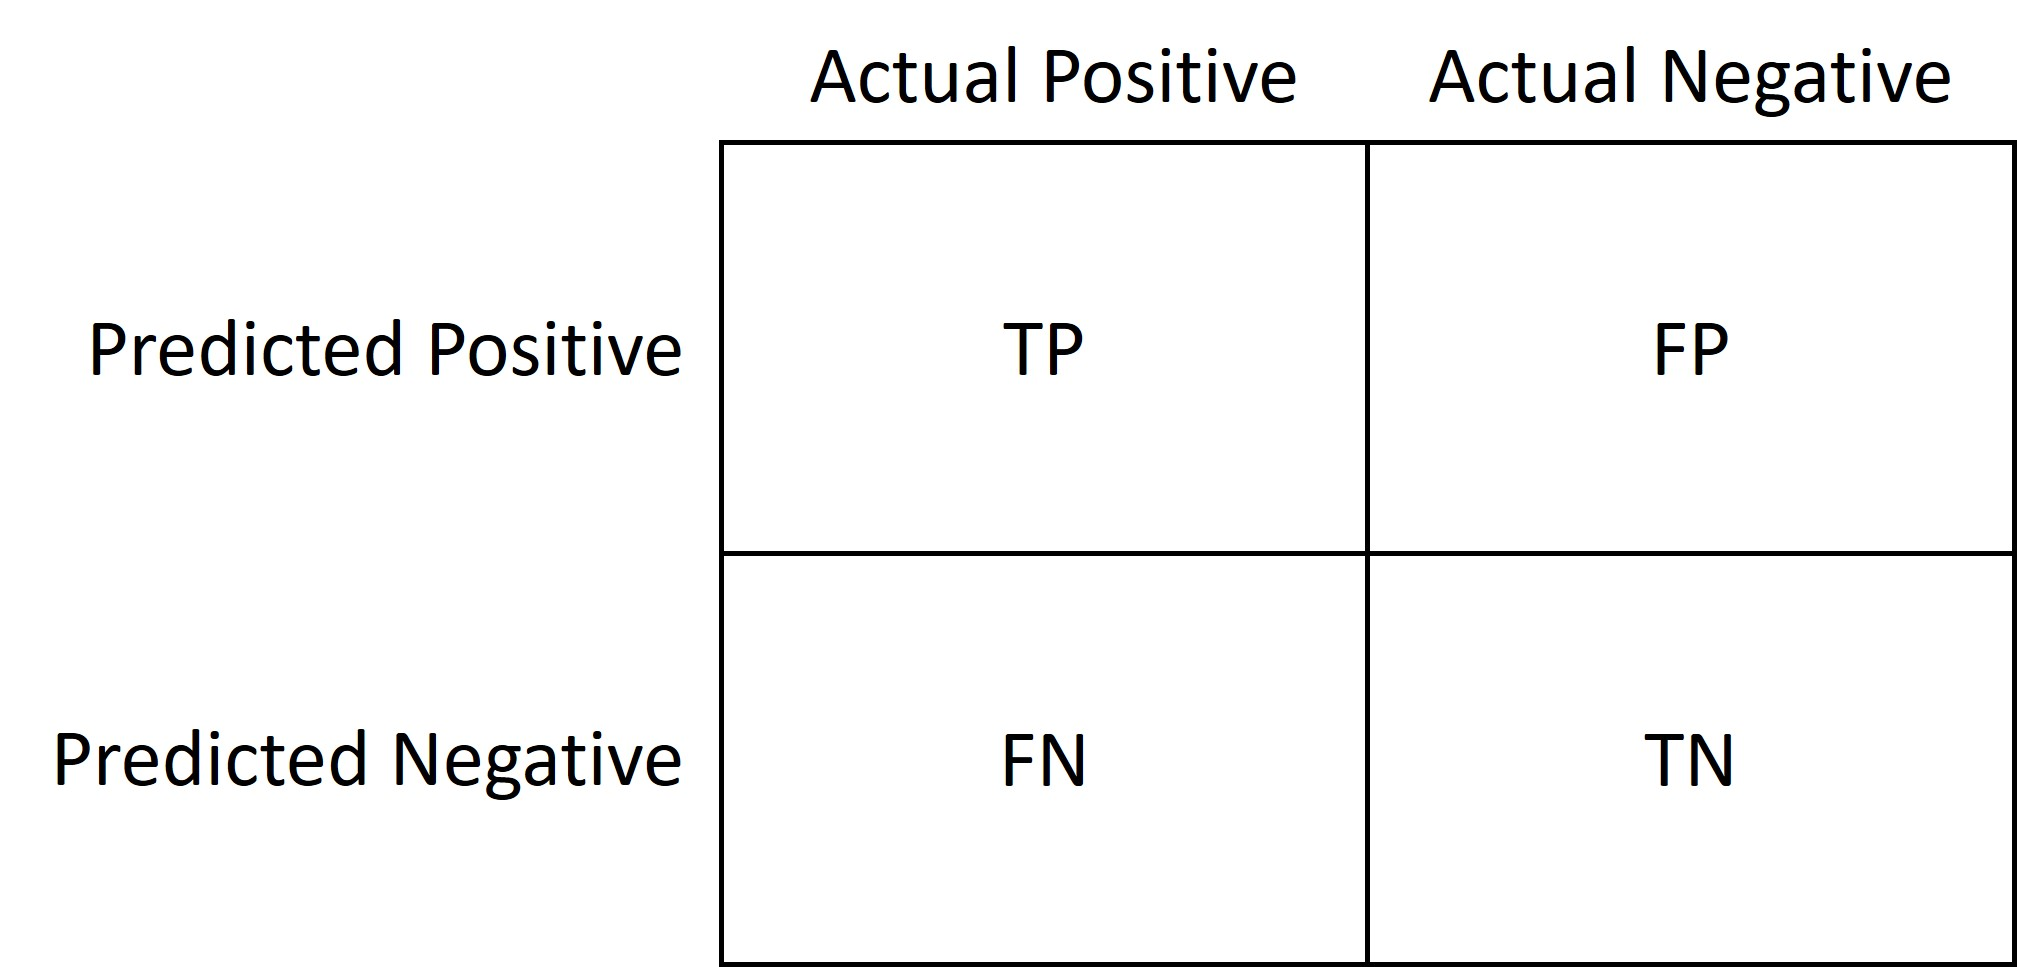
\includegraphics[width=0.75\textwidth]{3/figures/conf_matrix.jpg}
		\caption[Matriz de Confusión]{Matriz de Confusión. \\
		Fuente: Elaboración propia.}
		\label{3:fig302}
	\end{center}
\end{figure}

La matriz consta de cuatro partes importantes: TP, FP, FN y TN. Estos serán usados para presentar las fórmulas de las métricas más adelante. El primero (TP o true positive) se refiere a la cantidad de observaciones que se han predicho como positivos y que en verdad sí son positivos; por el contrario, FP (false positive) se refiere a aquellas predicciones dadas como positivos, pero en verdad son negativos. FN (false negative) es la cantidad de observaciones predichas como negativas; sin embargo, estas en realidad son positivas. Finalmente, TN (true negative) es la cantidad de observaciones predichas como negativas y que en realidad son también negativas.

A continuación, se presenta las métricas para medir el desempeño de la clasificación del modelo.

El accuracy representa aquella proporción del total de predicciones que se ha obtenido correctamente \parencite{ws_izco2018bdcp}. Este se calcula a través de la siguiente fórmula 1.

%\begin{equcaption}[!ht]
\begin{equation}\label{eq:accuracy}
\phantomsection
accuracy=\frac{TP+TN}{TP+TN+FP+FN}
\end{equation}
\myequations{Fórmula para calcular el accuracy}

El recall representa la proporción de solo los positivos reales predichos de manera acertada \parencite{ws_izco2018bdcp}. Se calcula con la siguiente fórmula.

%\begin{equcaption}[!ht]
\begin{equation}\label{eq:recall}
\phantomsection
recall=\frac{TP}{TP+FN}
\end{equation}
\myequations{Fórmula para calcular el recall}

Precision representa aquella proporción de lo predicho positivamente que es positiva \parencite{ws_izco2018bdcp}. Se calcula con la fórmula a continuación.

%\begin{equcaption}[!ht]
\begin{equation}\label{eq:precision}
\phantomsection
precision=\frac{TP}{TP+FP}
\end{equation}
\myequations{Fórmula para calcular el precision}

\begin{landscape}
	\section{Cronograma de actividades y presupuesto}
	Se propuso un cronograma para la investigación. Conforma desde el inicio hasta ser terminada con la sustentación final planeada para mediados del año 2024. Este se presneta en la Figura \ref{3:fig303}.

	\begin{figure}[!ht]
		\begin{center}
			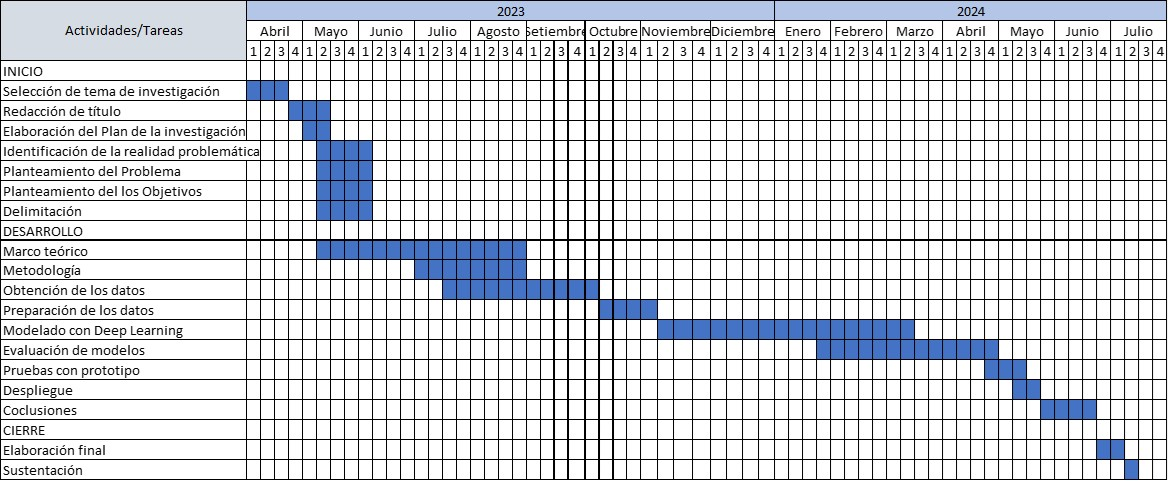
\includegraphics[width=1.50\textwidth]{3/figures/cronograma_tesis_thyr.jpg}
			\caption[Cronograma de actividades]{Cronograma de actividades.\\
				Fuente: Elaboración propia.}
			\label{3:fig303}
		\end{center}
	\end{figure}
	
\end{landscape}

Además, se determinó el presupuesto necesario para la elaboración completa de la investigación. Este se presenta en la Tabla \ref{3:table1}.

\begin{table}[H]
	\caption[Presupuesto]{Presupuesto.}
	\label{3:table1}
	\centering
	\small
	\begin{tabular}{llll}
		\specialrule{.1em}{.05em}{.05em}
		{Grupo} & {Item} & {Costo (soles)} & {Subtotal} \\
		\specialrule{.1em}{.05em}{.05em}
		\multirow{2}{4cm}{Recursos materiales} & {Laptop} & {S/ 6,500.00} & {} \\
		{} & {Materiales de escritorio} & {S/ 100.00} & {S/ 6,600.00} \\
		\cline{1-4}
		\multirow{2}{4cm}{Software y trámites} & {Matrícula de Trabajo de Tesis II} & {S/ 375.00} & {} \\ % & {Reserva de tema} & {S/ 2,700.00} & {} \\
		{} & {Cuotas de Trabajo de Tesis II} & {S/ 1,044.00} & {} \\
		%{} & {Derecho de inscripción} & {S/ 800.00} & {} \\
		%{} & {Derecho de sustentación} & {S/ 1,500.00} & {} \\
		{} & {Software} & {S/ 50.00} & {} \\
		{} & {Renta de servidor en la nube} & {S/ 224.15} & {S/ 1,693.15} \\ % & {S/ 5,274.15} \\
		\cline{1-4}
		\multirow{2}{4cm}{Extras} & {Consultorías} & {S/ 100.00} & {} \\
		{} & {Movilidad} & {S/ 200.00} & {S/ 300.00} \\
		\specialrule{.1em}{.05em}{.05em} 
		{} & {Total} & {} & {S/ 8,593.15} \\ % & {S/ 12,174.15} \\
		\specialrule{.1em}{.05em}{.05em}
	\end{tabular}
	\begin{flushleft}	
		\small Fuente: Elaboración propia.
	\end{flushleft}
\end{table}



